\chapter{Metode de experimentare}

După ce am prezentat toate componentele unui sistem de experimentare, am observat faptul că singura componentă ce determină distribuția entităților în cadrul unui experiment, dar și efectele pe care le are serviciul, fața de aplicația principală, este aceea de \textit{Assigner}. Reamintim că prin intermediul funcției \textit{AssignGroup}, ce primește ca parameterii identificatorul unei entități și decrierea completă a unui experiment, vom returna identificatorul grupului din care va face parte entitatea. 

Vom studia inițial modul în care vom determina diferențele între două grupuri, urmând ca mai apoi să prezentăm câteva mecanisme de experimentare. Le vom testa mai apoi practic, ilustrând metodologia, și modul de evaluare al acestora.

\section{Analiza experimentelor}

Scopul final al unui sistem de experimentare este acela de a obține o viziune de ansamblu asupra diferitelor abordări posibile, pentru a putea mai apoi decide care dintre acestea este cea mai profitabilă pentru produsul respectiv. De aceea, un aspect vital este acela de a cuantifica aceste diferențe. Vom considera, o convenție, că vor exista mai multe grupuri, și dorim să aflăm care este cel mai profitabil, prin prisma mediei unei metrice. De asemenea, vom considera că va exista întotdeauna un grup de control, ce va cuantifica valoarea actuală a metricei, în stadiul curent al aplicației. Vom calcula astfel diferența între fiecare grup experimental și cel de control în ceea ce privește media metricei alese.

Vom da un exemplu pentru a putea înțelege mai bine abordarea pe care o avem. Presupunem că avem un produs de comerț online, și există 3 grupuri: \textit{control}, \textit{test1} și \textit{test2}, iar metrica ce ne interesează este rata conversiilor în aplicația respectivă. Vom compara media ratei conversiilor pentru grupurile \textit{test1} și \textit{test2} cu media ratei conversiilor pentru grupul de control.

\begin{theorem}
	\index{metrica}
	Media unei metrici pentru o populație este distribuită normal, de medie ${\mu}$ și deviație standard $\frac{\sigma}{\sqrt{n}}$, unde $n$ reprezintă numărul observațiilor, conform \textbf{teoremei limită centrală}.
\end{theorem}

Prin convenție, în această secțiune ne vom referi doar la două grupuri, \textit{control} și \textit{test}, fără pierderea generalității, deoarece modul de comparare rămâne universal valabil.

\subsubsection{Notații}

Vom nota cu  $\mu_{control}$ și $\mu_{test}$, media metricei pentru \textit{\textbf{populația}} grupului de control, respectiv de test. În mod analog, vom nota cu $\sigma_{control}$ și $\sigma_{test}$, deviația standard a metricei pentru \textit{\textbf{populația}} grupurilor. Pentru a nota media \textbf{observațiilor} metricei pentru cele două grupuri vom folosi simbolurile $\overline{X}_{control}$, respectiv $\overline{X}_{test}$, în timp ce pentru deviația standard a observațiilor vom folosi $s_{control}$ și $s_{test}$. Nu în ultimul rând vom nota cu $N_{control}$ și $N_{test}$ numărul de observații din grupul de control, respectiv test.

\subsubsection{Testul Welsch \textit{t}}

Pentru efectuarea comparației vom calcula intervalul de încredere pentru diferentă între $\mu_{control}$ șî $\mu_{test}$. Pentru acest lucru vom folosi testul statistic \index{testul Welsch} \textit{Welsch} \cite{Welch1947}. Testul \textit{Welch} este un test pentru două eșantioane, folosit pentru a testa ipoteza că aceastea au aceeași metrică. 

Testul \textit{Welch t}, este o adaptare a testului \textit{Student t}, acesta având la bază testul Student. Reamintim cititorului că testul student este folosit pentru a determina dacă mediile a două populații sunt diferite. Testul Welch este însă mult mai robust când cele două eșantioane au deviații standard diferite, dar și dimensiuni diferite. Acest tip de teste se efectuează de obicei în practică când cele două eșantioane nu se suprapun, și de aceea se pretează excelent pentru a fi folosit de către un sistem de experimentare. 

Vom expune modul de calcul al testului, dar și cum putem calcula intervalul de încredere pentru diferența dintre media metricei între grupul de test și grupul de control.

Pentru a efectua testul statistic \textit{Welsch}, va trebui să calculăm statistica \textit{t}\cite{Welch1947}, astfel:

\begin{equation}
\label{tstatistic}
	t = \frac{\overline{X}_{test} - \overline{X}_{conrol}}{
		\sqrt{ {\frac{s_{test}^2}{N_{test}} }+ {\frac{s_{control}^2}{N_{control}}}}
		}
\end{equation}

\vspace{0.8cm}

Pentru a determina gradele de libertate vom folosi o ecuație pentru aproximarea acestora, ce poartă numele de ecuația \index{Welch–Satterthwaite}\textit{Welch–Satterthwaite}\cite{Welch1947}. Astfel, $\nu$ se aproximează astfel:

\index{grade de libertate}
\begin{equation}
\label{vapprox}
\nu = \frac{({\frac{s_{test}^2}{N_{test}} }+ {\frac{s_{control}^2}{N_{control}}}) ^ 2}{
	\frac{s_{test}^4}{N_{test}^2 \nu_{test}} + 
	\frac{s_{control}^4}{N_{control}^2 \nu_{control}}
}
\end{equation}

\vspace{0.8cm}

În ecuația \ref{vapprox} am notat cu $\nu_{test} = N_{test} - 1$, gradele de libertate asociate primei estimări a varianței,  și $\nu_{control} = N_{control} - 1$, gradele de libertate asociatei estimării varianței pentru grupul de control.

O dată ce avem calculate statisticile $t$ și $\nu$, putem folosi distribuția \textit{t}, pentru a testa ipoteza nulă, conform căreia cele două medii ale populațiilor sunt egale, sau ipoteza alternativă că una din populații are media mai mare sau egală cu cealaltă, folosind un test cu coadă simplă, și de aici putem obține valoarea pentru \textit{p-value}, tocmai pentru a putea oferi utilizatorilor o interpretare mai ușoară a testelor.

\begin{remark}
	Aproximarea gradelor de libertate se face prin rotunjirea în jos a valorii obținute din relația \ref{vapprox}.
\end{remark}

Am descris astfel modul de comparare a mediilor unei metrice pentru două grupuri de testare diferite. Rămâne să expunem modul de calcul al intervalelor de încredere pentru diferența mediilor, pentru o precizie $\alpha \in (0, 1)$. Avem următoarea formulă de calcul: \cite{miao}

\begin{equation}
\label{interval}
\overline{X}_{text} - \overline{X}_{control} \pm t_{1 - \alpha/2, \nu} \
\sqrt{ {\frac{s_{test}^2}{N_{test}} }+ {\frac{s_{control}^2}{N_{control}}}}
\end{equation}

\vspace{0.8cm}

Menționăm ca $\nu$ se calculează de asemenea cu formula Welch-Satterthwaite.

Am expus astfel în această secțiune mecanismele statistice prin intermediul cărora vom compara o metrică pentru două grupuri. Prin convenție, datorită faptului că metoda descrisă are avantajele expuse, o vom utiliza implicit pe întreg parcursul lucrării.

\section{Preliminarii}

Având în vedere că în această secțiune vom prezenta mai multe moduri de experimentare, și implicit mai multe strategii, avem nevoie de instrumentele teoretice necesare pentru a cuantifica eficiența acestora.

\begin{remark}
	Problema minimizării unei metrice $M$, este echivalentă cu problema maximizării metricei $-M$.
\end{remark}

Astfel, vom considera prin convenție faptul că va trebui să maximizăm valoarea unei metrice.


Presupunem că există $n$ grupuri în experimentul nostru, și dorim să maximizăm o metrică. Vom nota cu $\mu_1, \mu_2, ... \mu_n$ valorile medii ale metricei pe care o monitorizăm în cele $n$ grupuri. Vom nota cu $\mu^*$ valoarea media optimă a metricei. Se poate observa relația:

\[
\mu^* = \max_{i = \overline{1, n}}\{\mu_i\}
\]

Fie momentul $t$ ce va reprezenta asignarea a celei de-a $t$ entități către un grup. Vom nota cu $r_t$ valoarea metricei obținută prin asignarea efectuată..

\begin{definition}
\index{regret}
\label{regret}
Vom defini regretul, în mod normal cu următoarea formulă: 
\[
\rho = T * \mu^* - \sum_{i = 1}^{T}{r_i}
\]
\end{definition}

\begin{definition}
\index{regretul mediu}
\label{regretaverage}
	Vom defini regretul mediu, pe care îl vom nota cu $\overline{\rho}$ astfel:
	\[
	\overline{\rho} = \frac{\rho}{T * \mu*} = 1 - \frac{1}{T * \mu^*}\sum_{i = 1}^{T}{r_i}
	\]
\end{definition}

\begin{remark}
	Regretul mediu cuantifică media regretului la fiecare iterație.
\end{remark}

\begin{definition}
	O strategie se va numi optimă dacă $\rho$, regretul asociat, este 0 la oricare moment de timp $t$.
\end{definition}

\begin{definition}
\index{zero-regret}
	O strategie se va numi strategie "zero-regret", dacă valoarea medie a regretului, $\overline{\rho}$ tinde către 0 cu probabilite 1, atunci când $t \to \infty$.
\end{definition}

\begin{remark}
	O strategie de tipul "zero-regret" va converge către o strategie optimă după un anumit număr de runde.
\end{remark}

În literatură au fost descrise un număr larg de diferite strategii de selecție ce au ca scop minimizarea regretului. Cu toate acestea, pentru un sistem de experimentare există o altă metrică care este foarte importantă. Presupunem că există două grupuri pentru care valoarea medie a metricei pentru populația acestora este $\mu_1 \neq \mu_2$.

\begin{definition}
	\index{timp de convergență}
	Vom nota cu $T_{\alpha}^*$ numărul de asignări după care am obținut rezultate semnificative din punct de vedere statistic, cu încredere $\alpha$, că mediile celor două grupuri sunt diferite. Vom denumi această metrică pe care lucrarea o propune, \textbf{timpul de convergență}, sau durata de convergență.
\end{definition}

\section{Testare A/B}

Există mai multe metode de experimentare, dar care cea mai uzitată în industria informatică este de departe aceea a testării \textit{A/B}, ea fiind folosită în mod constant de companii precum \textit{Google}, \textit{Facebook}, sau \textit{Amazon}. 

\begin{definition}
	\index{testare A/B}
	\textbf{Testarea A/B} este o formă de testare a ipotezelor statistice, ce implică existența a două grupuri, unul de control și unul de test, iar între acestea două diferă valoarea unei singure variabile.
\end{definition}

Testarea \textit{A/B} este una din cele mai răspândite metode de experimentare datorită simplității acesteia. Pentru a înțelge mai bine modul în care se folosește aceasta vom da un exemplu. Vom presupune că un magazin de comerț on-line dorește să determine care culoare este mai potrivită pentru butonul de finalizare comandă. Se creează astfel două grupuri de utilizatori, primul grup va observa un buton roșu, în timp ce al doilea grup va observa un buton verde. Apoi se adună date referitoare la media CTR\footnote{Click through rate}-ului fiecărui grup până când se va observa o diferența seminificativă din punct de vedere statistic. Astfel, se va alege culoarea butonului ce va facilita obținerea unor rezultate mai bune. 

\begin{remark}
	Deși în mod istoric, în contextul testării A/B avem două grupuri, putem extinde metoda pentru a testa mai mult de 2 valori ale unei singure variabile.
\end{remark}

Această abordare este folosită de multe ori pentru modificări incrementale, și astfel grupul de control nu va observa nicio modificare asupra produsului, în timp ce grupul de test va observa diferențele cauzate de o valoare diferită a unei variabile. Deși poate părea ca este un concept foarte simplu, această metodă este foarte puternică. Pentru a putea obține rezultate semnificative din punct de vedere statistic cât mai repede, se recomanda ca metricele pe care dorim să le cuantificăm să fie în număr cât mai mic, la fel precum numărul de variații ale variabilele alese pentru testare.

\begin{remark}
	Deși se pot obține rezultate semnificative foarte rapid, este necesar ca un experiment să fie derulat cel puțin pe parcursul unei săptămâni întregi, dacă nu mai mult, pentru a se limita efectul de sezonalitate.
\end{remark}

O limitare evidentă a testării A/B este aceea că ne aflăm în imposibilitatea de a testa diferite valori pentru mai multe variabile și să cuantificăm efectul acestora, cât șî corelațiile acestora. De aceea a fost dezvoltat mecanismul de \textbf{\textit{testare cu variabile multiple}}. El este bazat pe aceeași idee centrală precum testarea A/B, însă permite modificarea mai multor variabile simultan. Deși poată parea mai atractivă, această metodă are nevoie de un \textit{eșantion} mult mai mare pentru a aduna date seminificative din punct de vedere statistic, și de aceea nu este practică pentru produsele software ce nu se bucură de o popularitate deosebită. De asemenea, mecanismul de cuantificarea al efectelor este unul mult mai complex. Această metodă nu este folosită extensiv în industrie, și de aceea lucrarea nu va insista să o descrie, deși sugerează cititorului consultarea \cite{johnson1992applied} pentru mai multe detalii.

\subsection{Asignarea entităților}

În cele ce urmează vom detalia modul în care sunt asignate entități către grupurile participante la test.

\begin{remark}
	Testarea de tip A/B nu se efectuează pe întrega populație ci doar pe o parte a acesteia.
\end{remark}

Motivul pentru care acest lucru se întâmplă este unul foarte simplu. Se dorește ca prin limitarea expunerii populației să se obțină date semnificative din punct de vedere statistic, dar să se construiască în același timp o limită superioară redusă pentru posibilele efecte negative ale experimentului. Se va asocia identificatorului fiecărei entități, în mod deterministic, un număr natural, iar apoi se va folosi acesta, împreună cu un \textit{seed}\footnote{O valoare aleatorie fixată} pentru a se determina dacă aceasta participă sau nu la experiment.

\begin{remark}
	Pentru transformarea indentificatorului unei entități într-un număr se va folosi o funcție de dispersie.
\end{remark}

Pentru testarea A/B se vor specifica de la începutul experimentului, \textit{în mod static}, dimensiunile grupurilor participante. Vom nota cu $frac_{i}$ fracția participanților la experiment ce vor fi asignați către grupul $i$.

 Un mod foarte utilizat de partiționare a experimentului în grupuri, este ca fiecare dintre acestea să aibe o pondere egală în întreg experimentul. Deoarece această abordarea este standard folosită în industrie pentru astfel de experimente, o vom folosi pe întreg parcursul lucrăii raportându-ne la aceasta. Avantajele unei astfel de metode sunt simplitatea, atât pentru înțelegerea experimentului, cât și pentru implementarea acestuia.

Pe de altă parte, abordarea statică are o serie de dezavantaje foarte mari. Cel mai mare dezavanataj este că nu e posibilă schimbarea distribuției grupurilor, și astfel nu se pot gestiona într-un mod inteligent efectele experimentului. 

\begin{remark}
	Strategia de partiționare folosită va avea un regret egal cu
	\[
	\rho = T ( \mu^*  - \sum_{i = 1}^{n} frac_{i} \overline{\mu_i})
	\]
\end{remark}

\begin{remark}
	Dacă fiecare grup va avea o pondere egală în cadrul experimentului vom avea:
	\[
	\rho = T ( \mu^*  - \frac{1}{n} \sum_{i = 1}^{n}\overline{\mu_i})
	\]
\end{remark}

De aceea, după cum am menționat, asignând fiecărui grup o pondere egală, se pot pierde oportunități importante, mai ales pentru aplicațiile software ce nu se bucură de un trafic foarte mare, sau se află la începutul dezvoltării unui produs. Vom propune un mod de testare alternativ, ce are o serie de avantaje, împreună cu câteva strategii dezvoltate pentru a utiliza cât mai bine ideile ce urmează a fi enunțate.

\section{Testare 'Multi-armed bandit'}

\index{multi-armed bandit}
Metoda de experimentarea pe care urmează să o prezentăm are ca inspirație problema probabilistică a banditului cu mai multe brațe, ce este tratată cu interes în mai multe lucrări de specialitate. În această problemă, un parior are în fața sa o serie de mașini electronice de jocuri de noroc. Acesta trebuie să decidă de câte ori să joace fiecare mașină și în ce ordine, astfel încât ascesta sa maximize potențialul câștig printr-o secventă de trageri de manetă. 

Se observă astfel o analogie cu problema ce presupune asignarea unor entități în anumite grupuri de experimentare. Astfel, putem reformula problema pentru a căuta o strategie optimă de asignare a entităților astfel încât să maximizăm efectele pozitive cutantificate prin prisma unei metrice, fiind echivalent cu minimizarea regretului definit anterior. De altfel, această metodă a fost folosită în studiile clinice pentru a minimiza pierderile asupra pacienților.

Există un număr de soluții convergent optime, însă complexitatea acestora este una substanțială. Pe lângă acest aspect, trebuie notat faptul că se urmărește doar minimizarea regretului, și nu se ține cont astfel de durata de convergență pentru a obține rezultate semnificative din punct de vedere statistic. 


Există un număr de soluții \textit{aproximative}, iar lucrarea le va aminti pe cele ce sunt viabile în contextul dat.

Vom descrie o serie de strategii semi-uniforme ce sunt bazate pe aceeași idee centrală, dar diferă prin detaliile de implementare. Se identifică două faze centrale, \textit{faza de explorare} și \textit{faza de exploatare}.

\index{faza de explorare}
\textbf{Faza de explorare} este o simulare cu abordarea propusă de testarea A/B. De altfel, numele acesteia provine din scopul ei de a aduna date referitoare la performanța fiecărui grup.

\index{faza de exploatare}
\textbf{Faza de exploatare} propune folosirea unor cunostințe acumulate din faza de explorare pentru a asigna entitățile către experimente într-un mod mai inteligent. Pentru strategiile următoare faza de explorare va consta în asignarea tuturor entităților către grupul cu cea mai bună performanță în faza de explorare.

\begin{itemize}
	\item \textbf{Epislon-Greedy}: Această strategie propune separarea entităților în două grupe, de proporție $\epsilon$ și $1 - \epsilon$, unde prima grupă va constitui faza de explorare iar cea de-a doua grupă va reprezenta faza de exploatare. Faza de exploatare și explorare se desfășoară în paralel.
	\item \textbf{Epislon-first}: Această strategie presupune introducerea primelor $\epsilon N$ entități în faza de explorare, urmate apoi de $(1-\epsilon)N$ entități ce fac parte din faza de exploatare, urmând ca apoi procesul să se repete. Astfel, faza de explorare și exploatare se desfășoară secvențial.
	\item \textbf{Epsilon-descrescător}: Este similară cu strategia \textit{Epsilon-Greedy}, dar propune scăderea termenului $\epsilon$ o dată cu creșterea dimensiunii experimentului.
	\item \textbf{Epsilon-contextual}: Similară cu strategia \textit{Epsilon-Greedy}, dar propune recalcularea factorului $\epsilon$ în funcție de contextul experimentului.
\end{itemize}

Menționăm că cea mai utilizată și indicată strategie pentru un sistem de experimentare este cea de tipul \textit{Epislon-Greedy}, sau \textit{Epislon-descrecător}. O problemă a celei din urmă este aceea că în cazul experimentelor ce vor fi desfășurate pe o perioadă de timp extinsă, pentru a elimina efectul de sezonalitate, faza de explorare va avea un rol neseminificativ în ultimele stagii, și astfel informațiile referitoare la grupurile care nu sunt foarte performante nu vor fi cu mult îmbunătățite, și în acest mod putem ajunge la o durată mai mare de convergență.

Pe lângă strategiile propuse anterior, există o \textbf{strategie probabilistică}. Aceasta propune o idee ingenioasă, conform căreia numărul de asginări către un anumit grup din cadrul experimentului ar trebui să reflecte probabilitatea ca acel grup să fie optim din punctul de vedere al metricii cuantificate. Această strategie mai poartă numele și de \textit{Bayesian Bandits}. Deși abordarea exploatează mai puțin informațiile acumulate, are avantajul de a acumula informații despre toate grupurile, la un ritm proporțional cu performanța acestora. Astfel, grupurile cele mai eficiente vor avea cele mai multe informații, iar acest fapt poate indica un timp de convergență mai scăzut decât pentru strategiile propuse anterior.

Vom analiza așadar, în cele ce urmează strategia \textit{Eplison-Greedy} și \textit{Bayesian Bandits}. Pe lângă acestea, \textbf{lucrarea propune o abordare alternativă,} hibridă între ideile prezentate, pentru a o obține un compromis optim între toate abordările. Fie $\epsilon, \beta \in(0, 1), \epsilon + \beta < 1$. Vom construi 3 grupe. Prima grupă va fi o grupă în care se va desfăsura faza de explorare în proprție constantă de $\epsilon$. În cea de-a doua grupă se va desfăsura faza de exploatare, în proporție de $\beta$. Ultima grupă va conține $1 - (\epsilon + \beta)$ din entitățile participante și va urma strategia probabilistică de asignare către grupurile experimentului. Toate cele 3 faze se vor desfășura în mod concurent.

Motivația ce a condus la dezvoltarea acestei idei este aceea că prin păstrarea unei faze de explorare constantă vom garanta posibilitatea de schimbare a rezultatelor experimentelor în cazul în care efectele se vor vedea doar după o durată lungă de timp. A doua fază, de exploatare ajută la echilibrarea regretului pierdut prin faza de exploatare, în timp ce abordarea probabilistică asigură un compromis optim între durata de convergența și valoarea regretului.

\section{Analiza strategiilor}

În secțiunea de fața vom analiza toate strategiile enumerate anterior, cuantificând metricele de regret, și timpul de convergență. Vom putea să determinăm astfel cât de eficiente sunt fiecare din aceste strategii: \textit{testare A/B}, \textit{Epsilon-Greedy}, \textit{Bayesian Bandit} și strategia hibridă propusă de lucrare, pe car eo vom numi \textit{Hybrid Bandit}. 

Vom presupune că vom avea de efectuat un experiment în care variem o singură valoare a unei variabile. De asemenea putem presupune, fără pierderea generalității că vom avea doar două grupuri, unul de control și unul de test. Am ales un astfel de cadrul simplificat pentru analiză, deoarece acesta este cel mai des folosit în practică, și permite cititorului să își formeze o viziune de ansamblu asupra metodelor utilizate. Folosind concluziile obținute într-un astfel de mediu se poate formula ușor o generalizare completă.

Ne amintim că am definit în ecuația \ref{interval} modalitatea de a afla intervalul de încredere corespunzător diferenței mediilor a două metrice. Pentru compararea diferitelor metode de asignare a entităților va trebui să comparăm durata de convergența și regretul. Folosind relațiile definite la începutul acestui capitol, putem să determinăm numărul mediu minim de iterații necesare, după care testul va converge și vom fi obținut rezultate semnificative din punct de vedere statistic. 

Presupunem că știm mediile \textit{populației}, dar și deviațiile standard ale acestora, $\mu_{control}, \mu_{test}$ respectiv $s_{control}, s_{test}$, pentru metricele monitorizate.

\begin{theorem}
	\label{widthobs}
	Dacă dimensiunea intervalului de încredere este mai mică decât diferența $|\mu_{control} - \mu_{test}|$, atunci testul va respinge ipoteza nulă, și va accepta ipoteza alternativă conform căreia cele două medii sunt diferite.
\end{theorem}

Din ecuația \ref{interval} deducem următoarea formulă: 

\begin{equation}
\label{width}
D =  t_{1 - \alpha, \nu} \sqrt{ {\frac{s_{test}^2}{N_{test}} }+ {\frac{s_{control}^2}{N_{control}}}}
\end{equation}

\begin{theorem}
	Se va folosi $ t_{1 - \alpha, \nu}$ și nu $ t_{1 - \alpha/2, \nu}$ pentru determinarea lungimii intervalului de încredere.
\end{theorem}

Considerând că din grupul de control vor face parte $\alpha N, \alpha \in (0, 1)$ entități, iar din grupul de test $\beta N, \beta \in (0, 1)$, unde $\alpha + \beta = 1$ și unde am notat $N = N_{test} + N_{control}$, vom putea rescrie ecuația \ref{width} astfel încât să determinăm numărul de iterații necesare minime, pentru a obține rezultate semnificative din punct de vedere statistic.

\begin{theorem}
	Putem determina valoarea medie a timpului de convergență cu ajutorul formulei:
\label{requiredsample}
\[
N =  \frac{
	t_{1 - \alpha, \nu}^2 (\alpha s_{test}^2 + \beta s_{control}^2 )
	}{
	D^2 \alpha \beta
	}
\]
\end{theorem}

\begin{proof}
	Vom pleca de la ecuația \ref{width}:
\[
D =  t_{1 - \alpha, \nu} \sqrt{ {\frac{s_{test}^2}{N_{test}} }+ {\frac{s_{control}^2}{N_{control}}}}
\]	

\[
D^2 =  t_{1 - \alpha, \nu}^2 ({\frac{s_{test}^2}{N_{test}} }+ {\frac{s_{control}^2}{N_{control}}})
\]	

\[
\frac{D^2}{ t_{1 - \alpha, \nu}^2 }= {\frac{s_{test}^2}{N_{test}} }+ {\frac{s_{control}^2}{N_{control}}}
\]	

Cum $N_{control} = \alpha * N$, și $N_{test}  = \beta * N$ avem:

\[
\frac{D^2}{ t_{1 - \alpha, \nu}^2 }= {\frac{s_{test}^2}{\beta N} }+ {\frac{s_{control}^2}{\alpha N}}
\]	

\[
\frac{D^2}{ t_{1 - \alpha, \nu}^2 }= \frac{\alpha s_{test}^2 + \beta s_{control}^2}{\alpha \beta N}
\]

\[
\frac{N D^2}{ t_{1 - \alpha, \nu}^2 }= \frac{\alpha s_{test}^2 + \beta s_{control}^2}{\alpha \beta}
\]

\[
N =  \frac{
	t_{1 - \alpha, \nu}^2 (\alpha s_{test}^2 + \beta s_{control}^2 )
}{
D^2 \alpha \beta
}
\]
\end{proof}

Am arătat astfel că dacă știm distirbuția de asignare a entităților în cele două grupuri, alături de cele informațiile legate de medie și deviație standard pentru metricele \textit{populațiilor}, putem determina numărul mediu de iterații după care vom atinge rezultate seminficative din punct de vedere statistic.

Pentru a compara două metode, va trebui să analizăm și regretul mediu al acestora. Ne amintim că am definit regretul în relația \ref{regret}. Deoarece vom folosi un experiment în care cuantificăm o metrică binară, putem rescrie formula astfel:

\begin{equation}
\label{particularregret}
	\rho = T \mu^* - T(\alpha \mu_{control}  +  \beta \mu_{test})
\end{equation}

Pentru a efectua o comparație obiectivă, ne vom folosi de valoarea medie a regretului, pe care din relația \ref{regretaverage} și \ref{particularregret} o putem scrie astfel: 

\begin{equation}
\label{particularregretaverage}
	\overline{\rho} = \mu^* - (\alpha \mu_{control}  +  \beta  \mu_{test})
\end{equation}

\begin{theorem}
\label{particularaverageregret}
	Dacă presupunem $\mu_{test} > \mu_{control}$, fără pierderea generalității, putem scrie formula regretului mediu astfel:
	
	\[
		\overline{\rho} = \beta (\mu_{test} - \mu_{control})
	\]
\end{theorem}

\begin{proof}
	
	\[
		\overline{\rho} = \mu^* - (\alpha \mu_{control}  +  \beta  \mu_{test})
	\]
	
	\[
	\overline{\rho} = (\alpha + \beta)\mu_{control} - (\alpha \mu_{control}  +  \beta  \mu_{test})
	\]
	
	\[
	\overline{\rho} = \beta (\mu_{control} - \mu_{test})
	\]
\end{proof}

\subsection{Rezultate}

Folosind rezultatele postulate de observațiile \ref{requiredsample}  și \ref{particularaverageregret}, vom construi o serie de grafice ajutătoare pentru a putea compara toate abordările descrise. Acestea ne vor ajuta să identificăm vizual avantajele și dezavantajale fiecăreia, și ne vor permite să concluzionăm mai apoi asupra celei mai potrivite strategii.

Atât pentru regret, cât și pentru timpul de convergență, vom utiliza grafice de tipul \textit{heatmap}\footnote{Diagramă colorată cu intensități diferite, în funcție de valoarea funcției}. Pe axa \textit{oy} vom reprezenta valoarea medie a metricei în grupul de test, în timp ce axa \textit{ox} va corespunde valorii medie a metricei pentru entitățile de control. De asemenea, vom folosi o reprezentare ce poartă numele de \textit{hexbin}, pentru a putea aggrega o serie de valori, sub forma mediei, ce se află în vecinătatea unui punct central.

\subsubsection{Testarea A/B}

În contextul definit anterior, vom avea dimiensiunile celor două grupuri egale, $1/2$, și vom obține un regret mediu dat de formula:

\[
	\overline{\rho}_{ab} = \frac{1}{2} * (\mu_{text} - \mu_{control})
\]
	
Se poate vizualiza foarte ușor modul în care funcționează regretul, dar și durata de convergență, în figura \ref{fig:ab_evaluation}

\begin{figure}[H]
	\centering
	\begin{subfigure}{.5\textwidth}
		\centering
		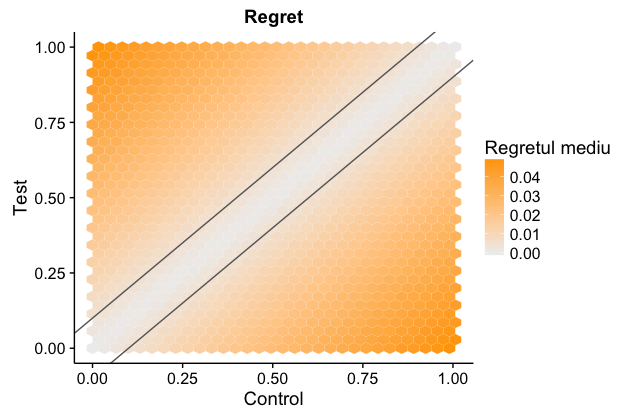
\includegraphics[width=1\linewidth]{ab_regret}
	\end{subfigure}%
	\begin{subfigure}{.5\textwidth}
		\centering
		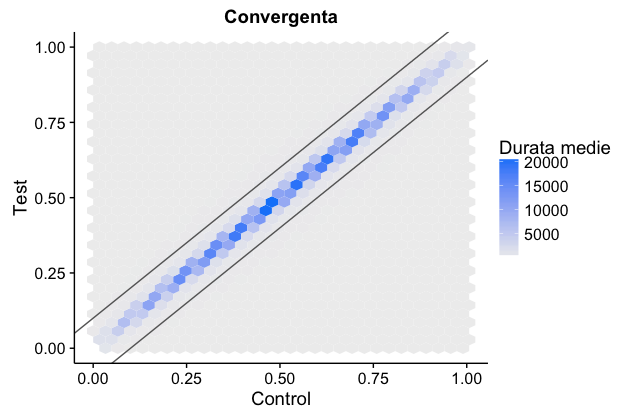
\includegraphics[width=1\linewidth]{ab_conv}
	\end{subfigure}
	\caption{Regretul și durata de convergența pentru testarea A/B\\}
	\label{fig:ab_evaluation}
\end{figure}

Se observă cum, atunci când cele două grupuri au valori ale metricelor cât mai apropiate, este necesar un număr mai mare de iterații pentru a putea determina din punct de vedere statistic că acestea sunt diferite. Pe de altă parte, datorită naturii statice a metodei de testare A/B, cu cât diferența dintre metrice este mai mare, se observă o corelație directă pozitivă cu regretul mediu.

\subsubsection{Greedy Epsilon}

Conform acestei strategii, regretul mediu va converge către următoarea formulă: \[
	\overline{\rho}_{\epsilon} = \frac{1}{2} \epsilon * (\mu_{text} - \mu_{control}) 
\]

Ținând cont de formula prezentată mai sus pentru regretul mediu al abordării testării A/B, se poate observa că obținem un factor de îmbunătățire egal cu $\frac{1}{\epsilon}$. Astfel, pentru $\epsilon = 0.1$ vom avea un regret mediu de 10 ori mai mic, iar acest fapt reprezintă un avantaj major pentru strategia de tip \textit{Greedy-Epsilon}. Pe de altă parte, vom examina diferențele în ceea ce privește timpii de convergența ai acestei strategii față de testarea A/B.

\begin{figure}[H]
	\centering
	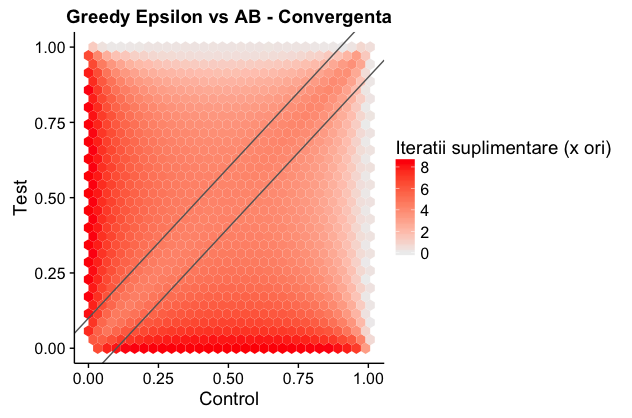
\includegraphics[max height=5cm,keepaspectratio]{ab_vs_epsilon_conv}
	\caption{Numărul de iterații necesare pentru convergență, cu metoda Greedy Epsilon, raportat relativ la testarea  A/B}
	\label{fig:ab_vs_epsilon_conv}
\end{figure}

În figura \ref{fig:ab_vs_epsilon_conv} se poate observa cum timpul de convergență a crescut de până la 8 ori, iar mediana creșterii este de \textit{4.24} ori. Astfel, se încetinește foarte mult iterarea rapidă asupra unui produs. 

\begin{remark}
	Vom folosi mediana și nu media pentru comparații pentru a putea evita efectul produse de \textit{outliere}\footnote{Valori ce sunt cu mult diferite de restul distribuției}
\end{remark}

Cum un experiment se efectuează oricum pe o parte din utilizatorii aplicației, lucrarea sugerează folosirea, în general, a testării A/B, înaintea strategiilor de tipul \textit{Greedy Epsilon}.

\subsubsection{Bayesian Bandit}

Reamintim că acest tip de strategie folosește informațiile \textit{a priori} despre mediile grupurilor pentru a determina modul de asignare a entităților. De aceea, regretul mediu va fi dat de formula 

\[
\overline{\rho}_{bayesian} = \frac{\mu_{control}}{\mu_{control} + \mu_{test}} * (\mu_{text} - \mu_{control})
\]

\begin{theorem}
	Regretul mediu pentru această strategie este întotdeauna mai mic decât regretul mediu pentru testarea A/B, $\overline{\rho}_{bayesian} < \overline{\rho}_{ab}$.
\end{theorem}


\begin{proof}
Cum am presupus fără pierderea generalității că $\mu_{test} > \mu_{control} \Rightarrow$

\[
\frac{\mu_{control}}{\mu_{control} + \mu_{test}} < \frac{\mu_{control}}{\mu_{control} + \mu_{control}} = \frac{1}{2} \Rightarrow
\]
\[
\overline{\rho}_{bayesian} < \overline{\rho}_{ab}
\]
\end{proof}


\begin{figure}[H]
	\centering
	\begin{subfigure}{.5\textwidth}
		\centering
		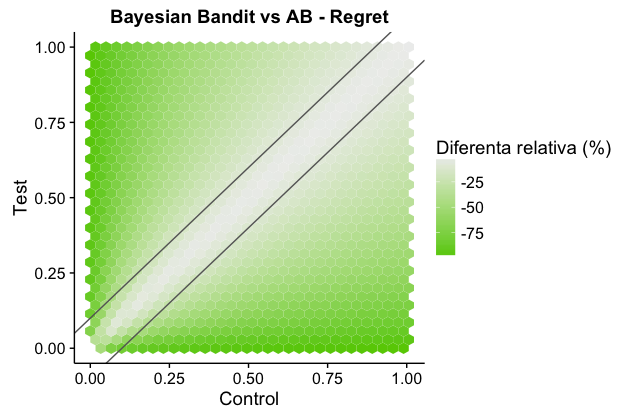
\includegraphics[width=1\linewidth]{ab_vs_bayesian_regret}
		\label{fig:sub1}
	\end{subfigure}%
	\begin{subfigure}{.5\textwidth}
		\centering
		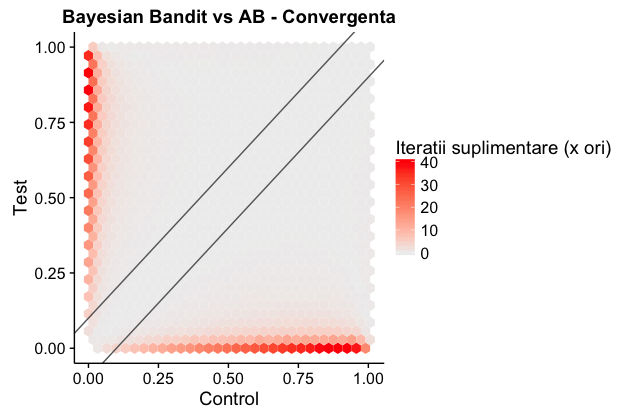
\includegraphics[width=1\linewidth]{ab_vs_bayesian_conv}
		\label{fig:sub2}
	\end{subfigure}
	\caption{Comparație relativă între Bayesian Bandit și testarea A/B}
	\label{fig:ab_vs_bayesian}
\end{figure}

Se poate observa în figura \ref{fig:ab_vs_bayesian}, optimizarea regretului ce are loc cu ajutorul acestei abordări. De altfel, mediana indică o optimizare cu \textit{33\%} a regretului. Pe de altă parte, numărul de iterații necesare pentru a obține convergența crește seminifcativ, însă doar pentru așa numitele \textit{edge-cases}, în care diferența între cele două grupuri este considerabilă. Mediana indică o creștere doar de \textit{0.06} ori a numărului de iterații necesar. Așadar, lucrarea propune utilizarea strategiei \textbf{Bayesian Bandit}, în detrimentul testării A/B.

\subsubsection{Hybrid Bandit}

Aceasta este abordarea alternativă, originală, pe care o propune lucrarea, și are ca scop eliminarea creșterii foarte mari a duratei de convergență pentru \textit{edge-cases}, păstrând în același timp avantajele aduse de abordarea descrisă sub numele de \textit{Bayesian Bandit}. Formula regretului este una mai complicată, dar care poate fi scrisă elegant ca o relație liniară între cele trei formule determinate anterior, astfel:

\[
\overline{\rho}_{hybrid} = \alpha * \overline{\rho}_{ab}  + \beta * \overline{\rho}_{\epsilon} + (1 - (\alpha + beta)) * \overline{\rho}_{bayesian} 
\]

În cazul curent, am ales $\alpha = \beta = 0.1$ pentru a fi consistent cu practicile cele mai uzitate în industrie.

\begin{figure}[H]
	\centering
	\begin{subfigure}{.5\textwidth}
		\centering
		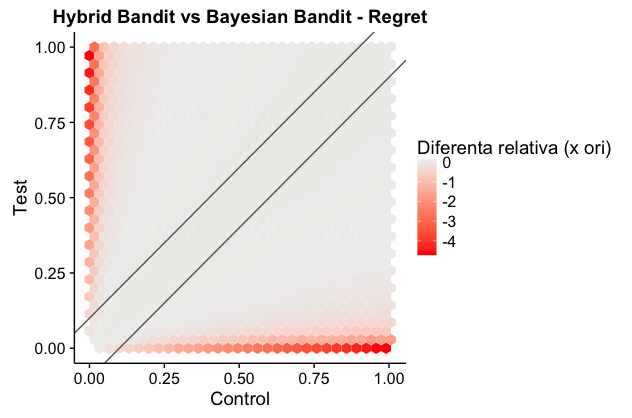
\includegraphics[width=1\linewidth]{hybrid_vs_bandit_regret}
	\end{subfigure}%
	\begin{subfigure}{.5\textwidth}
		\centering
		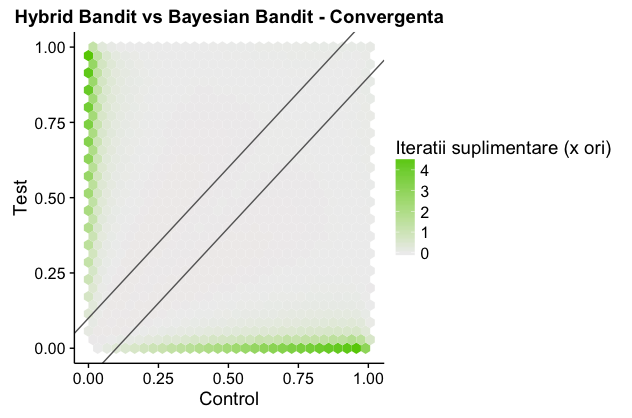
\includegraphics[width=1\linewidth]{hybrid_vs_bandit_conv}
	\end{subfigure}
	\caption{Comparație relativă între Hybrid Bandit și Bayesian Bandit}
	\label{fig:hybrid_vs_bayesian}
\end{figure}

Se poate observa în figura \ref{fig:hybrid_vs_bayesian} că, deși avem un regret mediu mai mare pentru acele \textit{edge cases}, se obține o durată de convergentă până la de 4 ori mai bună. Pentru restul cazurilor, cele două metode nu prezintă diferențe semnificative. Am reușit deci să adresăm problema obținerii rezultatelor seminificative pentru cazurile speciale.

\subsection{Concluzii}

Deși reprezintă un mecanism rudimentar, testarea A/B se comportă surprinzător de bine. Strategia de tip \textit{Greedy Epsilon} este una defectuoasă, cu o serie întreagă de lacune. \textit{Bayesian Bandit} reprezintă o abordare ingenioasă, ce se comportă mai bine decât testarea A/B în general, dar are probleme atunci când diferențele metricelor între cele două grupuri sunt foarte mari, din punctul de vedere al iterației de dezvoltare. 

În final, abordarea hibdridă, propusa de lucrare, prezintă un mecanism simplu, inegnios, și eficient în același timp, construind peste strategia descrisă de \textit{Bayesian Bandit}, adresând problemele legate \textit{edge cases}. De aceea, lucrarea consideră această metodă ca o alternativă general viabilă și validă, față de cele descrise în literatură.


